% !TEX program = xelatex
\documentclass[hyperref,a4paper,UTF8]{ctexart}
\usepackage[left=2.50cm, right=2.50cm, top=2.50cm, bottom=2.50cm]{geometry}
\usepackage[unicode=true,colorlinks,urlcolor=blue,linkcolor=blue,bookmarksnumbered=true]{hyperref}
\usepackage{latexsym,amssymb,amsmath,amsbsy,amsopn,amstext,amsthm,amsxtra,color,bm,calc,ifpdf}
\usepackage{graphicx}
\usepackage{enumerate}
\usepackage{fancyhdr}
\usepackage{listings}
\usepackage{multirow}
\usepackage{makeidx}
\usepackage{xcolor}
\usepackage{fontspec}
\usepackage{subfigure}
\usepackage{hyperref}
\usepackage{pythonhighlight}
\usepackage{float}
\usepackage{placeins}
\usepackage{graphicx}
\usepackage[zh-cn]{datetime2}  
\pagestyle{fancy}

\lstset{
    basicstyle=\ttfamily\small, % 等宽字体
    keywordstyle=\color{blue},    % 关键字颜色
    commentstyle=\color{green},   % 注释颜色
    numbers=left,                % 显示行号
    numberstyle=\tiny\color{gray}, % 行号样式
    frame=single,                % 边框
    breaklines=true,             % 自动换行
}

% 在这里填写页眉,可以选择三种对齐方式
\fancyhead[L]{}
\fancyhead[C]{\fangsong 软件测试与维护-大作业报告}
\fancyhead[R]{}

\begin{document}

% 封面页
\begin{titlepage}
    \begin{center}
        % LOGO
        \vspace*{2.0cm}
        %logo图片可以选择
        
\includegraphics[width=0.63\textwidth]{figures/南开logo.jpg}
        
        % 标题
        \vspace{4cm}
        \fontsize{28}{36}\selectfont
        {\heiti 《软件测试与维护》课程大作业报告} \\[0.5em]
        \fontsize{24}{26}\selectfont
        {\heiti Online-Boutique的部署、监控、维护\\ \& \\GDN论文复现}

        \vfill
        % 日期
        {\Large \today}
    \end{center}
\end{titlepage}


% 目录页
\newpage
\tableofcontents

% 正文内容
\newpage
\section{小组成员及分工}
\begin{table}[h!]
    \centering
    \begin{tabular}{|c|c|c|}
        \hline
        姓名 & 学号 & 分工 \\ 
        \hline
        李懋   & 2213189   & 项目负责人、微服务部署、论文算法复现(50\%)、实验报告撰写(50\%)+排版  \\ 
        \hline
        武英文   & 2211537   & 微服务部署、微服务测试   \\ 
        \hline
        陈瀚宇   & 2210590   & 微服务部署、ChaosMesh故障注入与监控(80\%)   \\ 
        \hline
        林诗润   & 2110637   & 微服务部署、实验数据收集、论文算法复现(50\%)   \\
        \hline
        于家齐   & 2212896   & 部分ChaosMesh故障注入与监控(20\%)、PPT制作   \\
        \hline
        黎思琪   & 2314313   & 实验报告撰写(50\%)   \\
        \hline
    \end{tabular}
    \label{tab:example_table}
\end{table}

\section{大作业成果}
\begin{itemize}
    \item 完成 Online-Boutique项目的部署、监控、维护
    \item 复现 GDN 图偏差网络论文算法
    \item 源代码仓库: https://github.com/lsroi/STM-CW
\end{itemize}

\section{实验概述}
本实验通过部署、监控、维护 Google 开源的微服务项目 Online-Boutique,深入理解微服务架构在云原生环境中的应用实践。相比传统的单体架构,微服务具备更强的灵活性、可扩展性和可维护性。本实验以一个完整的电商平台为载体,涵盖商品浏览、推荐、购物车、支付和发货等典型业务流程,涉及 Go、Java、Python、Node.js 等多语言服务.

实验基于 Minikube 构建本地 Kubernetes 环境,我们完成了从项目克隆、容器构建、服务部署到负载测试的全流程实践,学习了容器编排与服务治理。同时,我们借助 JMeter 和 Selenium 工具进行压力测试与自动化测试,评估系统在高并发下的稳定性与性能瓶颈。

在可观测性建设方面,我们引入 Prometheus 与 Grafana 实现服务监控与可视化,通过故障注入模拟真实运维场景,增强对系统韧性与可靠性的理解。此外,我们结合 GDN 图偏差网络算法的复现,探索智能化故障检测与异常分析方法,促进算法设计与工程实践的融合。


\section{实验环境}
\begin{itemize}
    \item 操作系统: macOS Sequoia 15.0 \& Windows 11
    \item Docker 28.0.4
    \item Minikube v1.35.0
    \item Git 2.39.5
    \item Selenium IDE 3.17.0
    \item JMeter 3.6.2
    \item Promethues v2.26.0
    \item Grafana 7.5.5
    \item PyTorch 1.5.1
    \item Python 3.6+
    \item CUDA 10.2
\end{itemize}

\section{微服务系统介绍}
项目Github仓库地址: https://github.com/JoinFyc/Online-Boutique
Online Boutique 是 Google 推出的一个典型微服务架构示例系统,具有完整的电商业务流程,包括商品展示、推荐、购物车、支付、发货、邮件通知等功能。Google 使用此应用程序来演示开发人员如何使用 Google Cloud 产品对企业应用程序进行现代化改造,这些产品包括:Google Kubernetes Engine (GKE)、Cloud Service Mesh (CSM)、gRPC、Cloud Operations、Spanner、Memorystore、AlloyDB和Gemini。此应用程序适用于所有 Kubernetes 集群。
\
该系统采用前后端分离设计,由 11 个微服务组成,使用多种语言开发,如 Go、Python、Node.js、Java 和 C#,这些服务之间通过高效的 gRPC 协议通信。系统中包括前端服务、商品目录服务、购物车服务、支付服务、货运服务、邮件服务、广告推荐服务、汇率转换服务、结账服务、推荐系统和负载生成器,每个服务独立部署、运行与扩展,具备良好的解耦性和可维护性。这种设计不仅能够提高开发效率,还支持异步扩展、容错恢复和弹性伸缩等微服务架构的核心优势。该项目高度还原了真实生产环境下的业务逻辑和服务依赖关系,是理解微服务架构、服务拆分与协同的重要实践案例。

\begin{figure}[H]
    \centering
    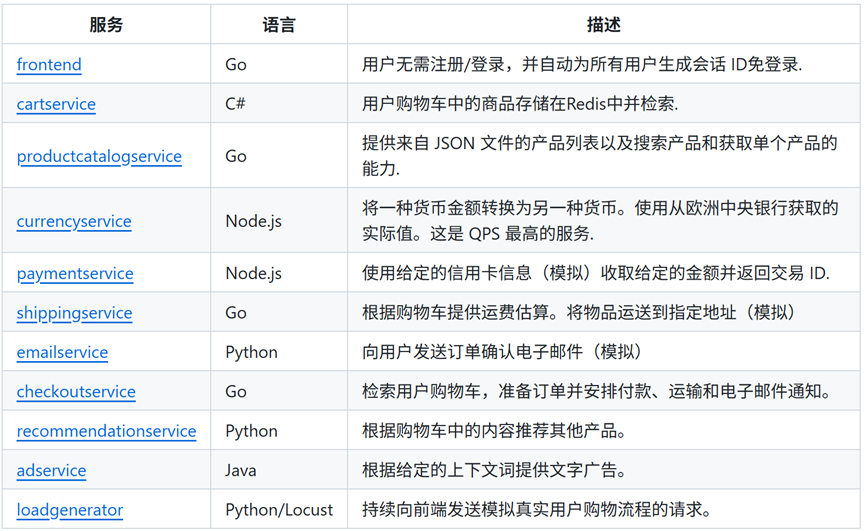
\includegraphics[width=0.75\linewidth]{微服务组成.png}
    \caption{微服务组成}
    \label{fig:enter-label}
\end{figure}
\begin{figure}[H]
    \centering
    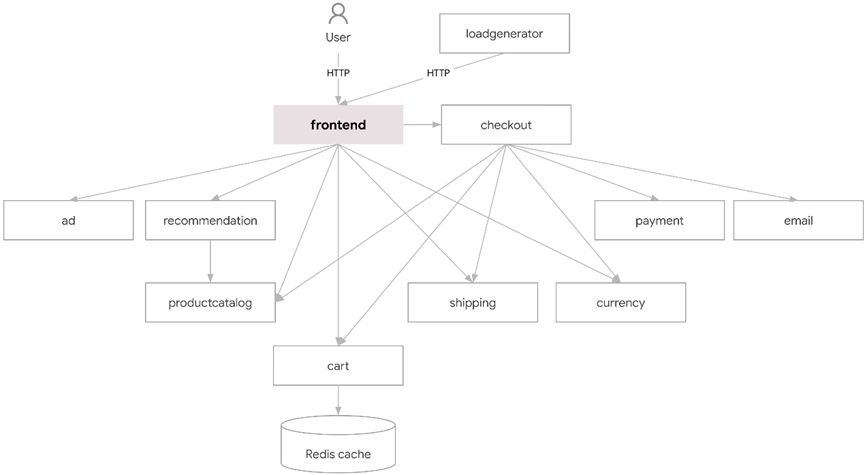
\includegraphics[width=1\linewidth]{微服务架构图.png}
    \caption{微服务架构图}
    \label{fig:enter-label}
\end{figure}

\section{微服务系统部署}
本实验采用 Minikube 在本地构建 Kubernetes 环境,实现对 Online Boutique 微服务系统的完整部署。首先,在本地环境中配置 Docker 和 Minikube,Docker 作为容器运行时,Minikube 作为单节点 Kubernetes 集群的模拟工具,能够帮助我们在本地完成容器化部署实验。安装完成后,使用如下命令启动本地集群,并设置合适的资源限制(如内存和 CPU),确保集群运行稳定:

拉取阿里云镜像
\begin{lstlisting}
    docker pull registry.cn-hangzhou.aliyuncs.com/google_containers/kicbase:v0.0.46
    docker tag registry.cn-hangzhou.aliyuncs.com/google_containers/kicbase:v0.0.46 kicbase:v0.0.46
\end{lstlisting}
\begin{figure}[H]
    \centering
    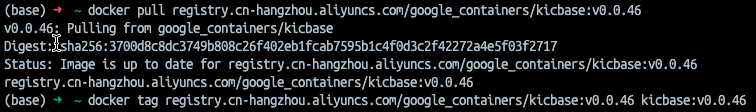
\includegraphics[width=0.75\linewidth]{部署/aliyun.png}
    \caption{拉取阿里云镜像}
    \label{fig:enter-label}
\end{figure}

启动Minkube
\begin{lstlisting}
minikube start # 启动minikube虚拟机,并在本地电脑上创建k8s集群
# 下面是可选的参数,可以根据具体情况选择
--driver=docker # 通常是默认配置
--cpus=4 # 分配4个cpu核心
--memory=6g # 分配6GB内存
--kubernetes-version=v1.35.0 # 启动指定版本的minikube集群
\end{lstlisting}
\begin{figure}[H]
    \centering
    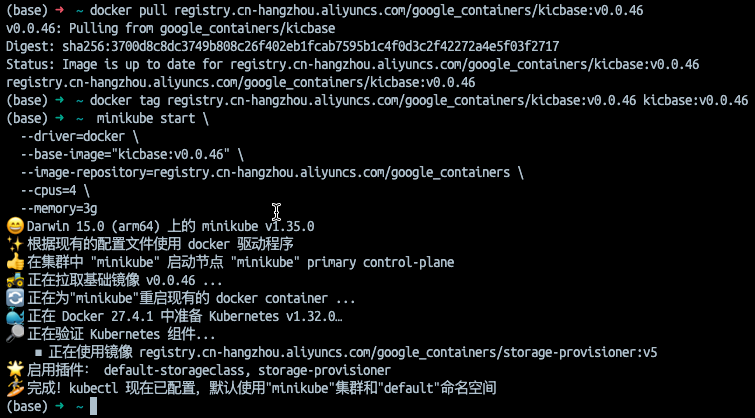
\includegraphics[width=0.75\linewidth]{部署/start.png}
    \caption{启动Minikube}
    \label{fig:enter-label}
\end{figure}

Git克隆项目
\begin{lstlisting}
git clone --depth 1 --branch v0 https://github.com/GoogleCloudPlatform/microservices-demo.git
cd microservices-demo/
\end{lstlisting}

\begin{figure}[H]
    \centering
    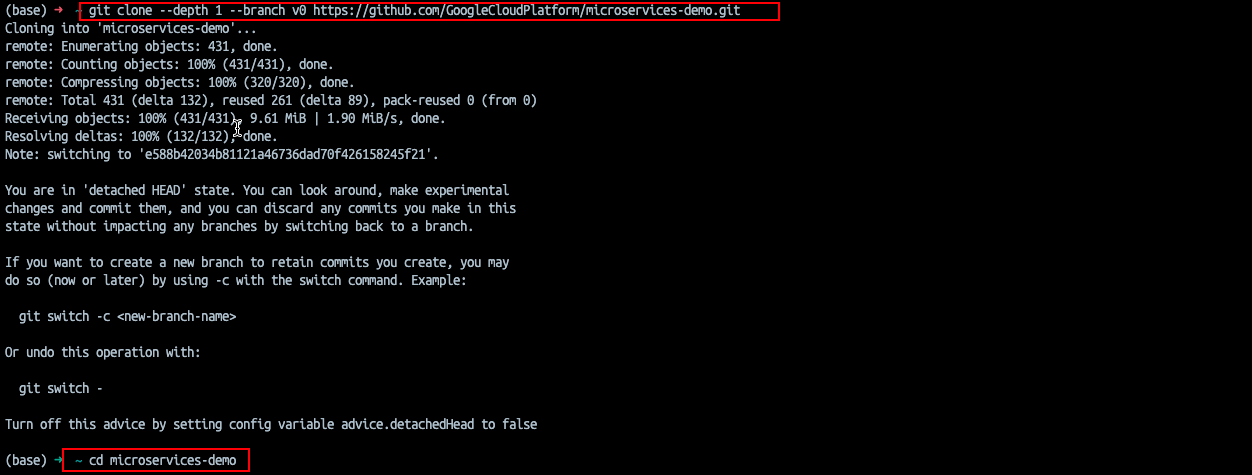
\includegraphics[width=0.75\linewidth]{部署/clone.png}
    \caption{clone项目}
    \label{fig:enter-label}
\end{figure}

部署所有服务: 
\begin{lstlisting}
kubectl apply -f ./release/kubernetes-manifests.yaml
\end{lstlisting}
\begin{figure}[H]
    \centering
    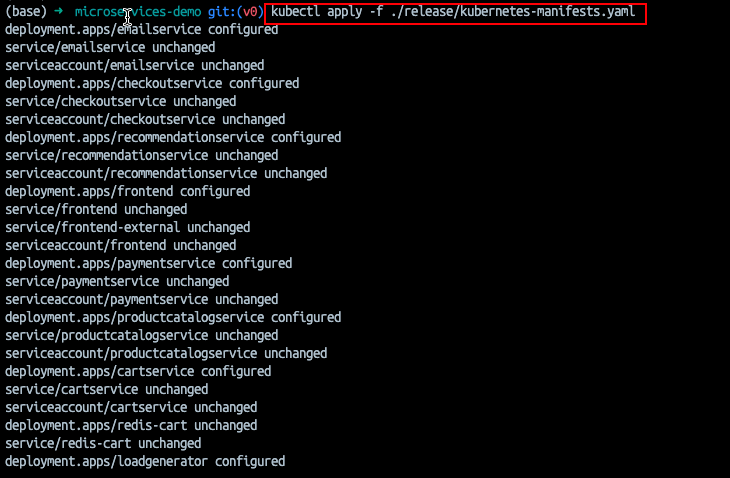
\includegraphics[width=0.75\linewidth]{apply.png}
    \caption{部署所有服务}
    \label{fig:enter-label}
\end{figure}

Kubernetes 会根据 YAML 文件中的定义拉取镜像、启动容器,并自动配置服务之间的依赖与通信。使用下列命令持续监控服务启动状态,此时确保所有 11 个微服务对应的 Pod 均若全部运行成功(处于Running状态),说明系统部署完成并已准备好对外提供服务
\begin{lstlisting}
kubectl get pods -M
\end{lstlisting}
\begin{figure}[H]
    \centering
    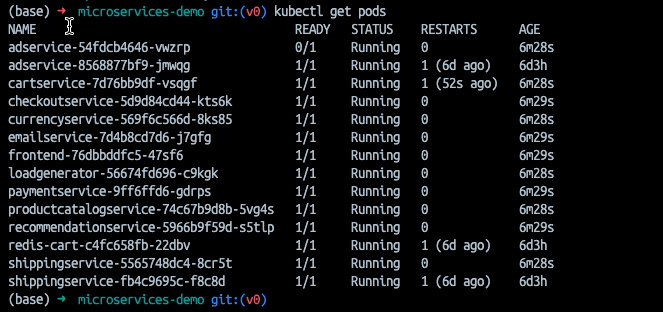
\includegraphics[width=0.75\linewidth]{部署/running.png}
    \caption{11个微服务状态}
    \label{fig:enter-label}
\end{figure}

获取前端服务的访问地址: 
\begin{lstlisting}
minikube service frontend-external
\end{lstlisting}
\begin{figure}[H]
    \centering
    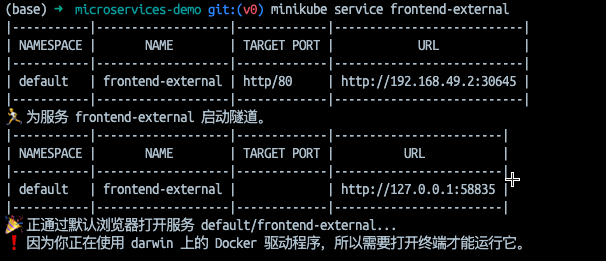
\includegraphics[width=0.75\linewidth]{部署/获取url.png}
    \caption{获取前端url}
    \label{fig:enter-label}
\end{figure}

前端效果图:
\begin{figure}[H]
    \centering
    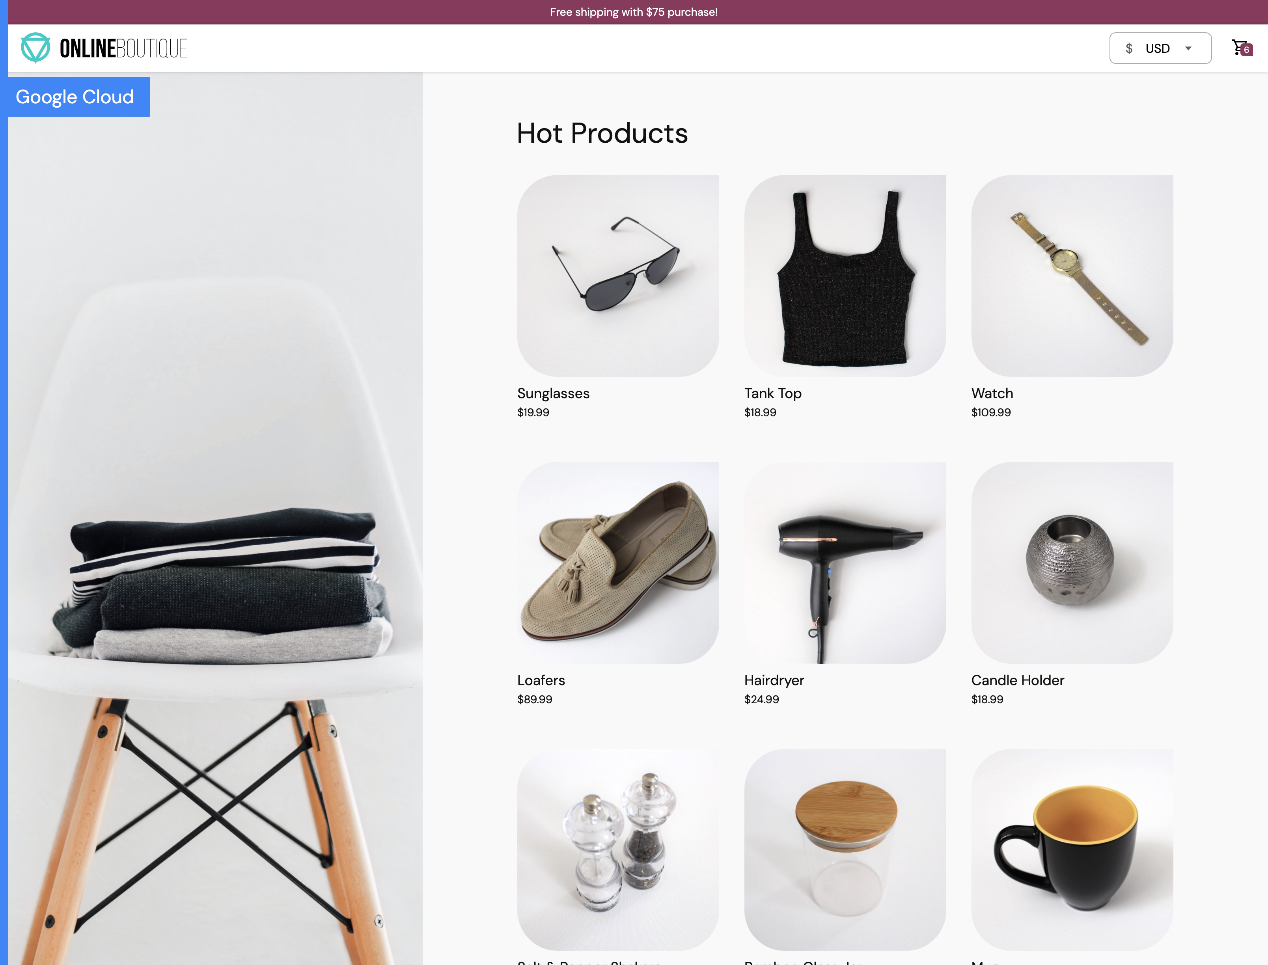
\includegraphics[width=0.75\linewidth]{部署/前端1.png}
    \label{fig:enter-label}
\end{figure}
\begin{figure}[H]
    \centering
    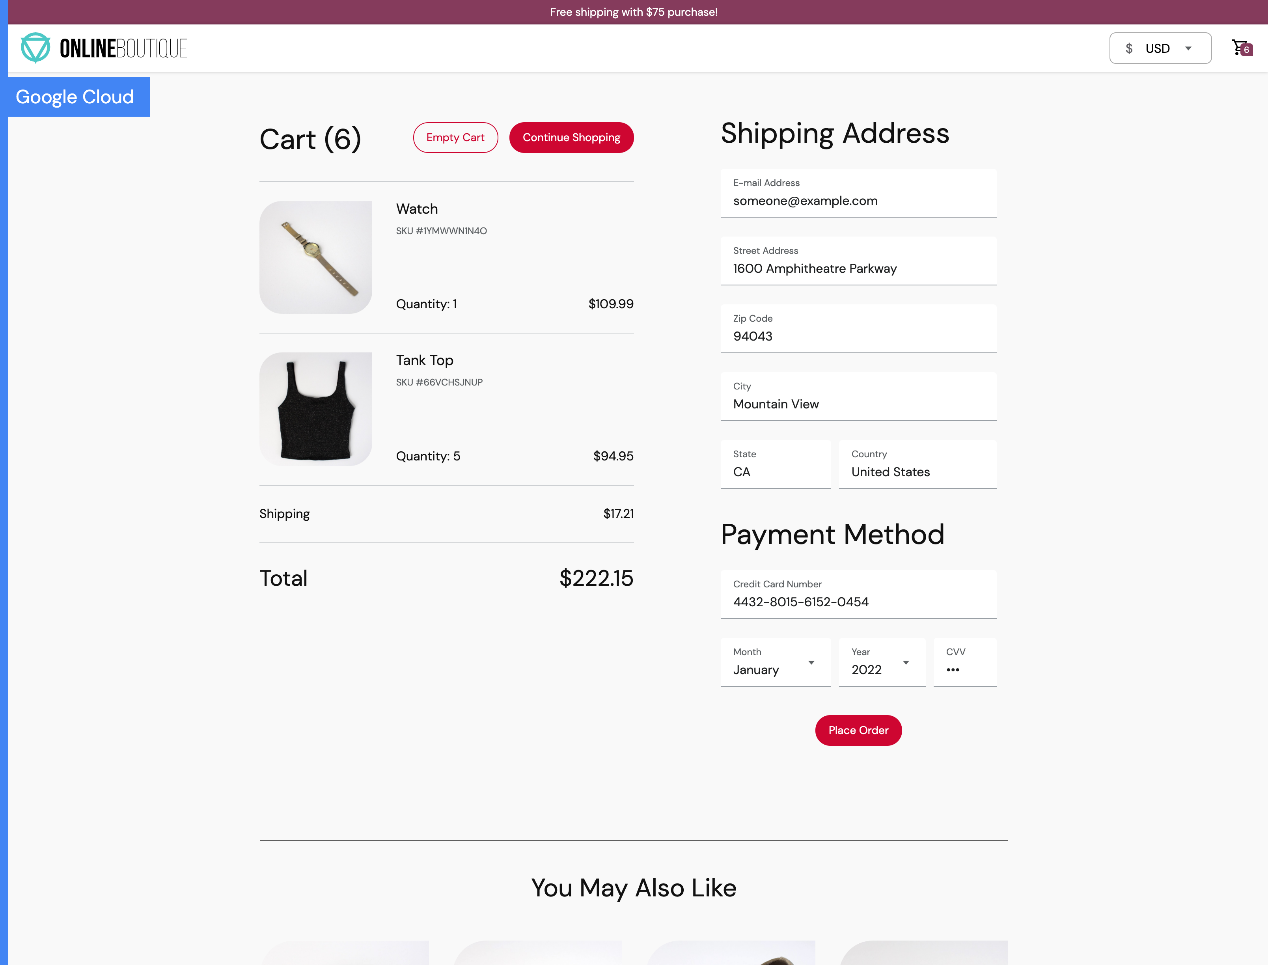
\includegraphics[width=0.75\linewidth]{部署/前端2.png}
    \label{fig:enter-label}
\end{figure}


\section{微服务测试}
部署完毕后,运行测试工具
\begin{figure}[H]
    \centering
    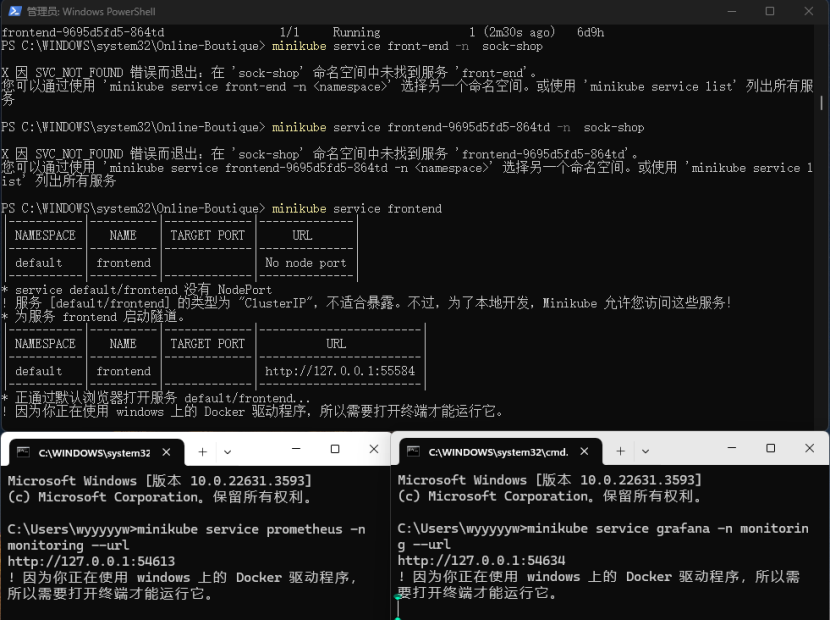
\includegraphics[width=0.75\linewidth]{测试/1.png}
    \caption{运行测试工具}
    \label{fig:enter-label}
\end{figure}
使用Selenium IDE录制测试过程,生成java脚本
\begin{figure}[H]
    \centering
    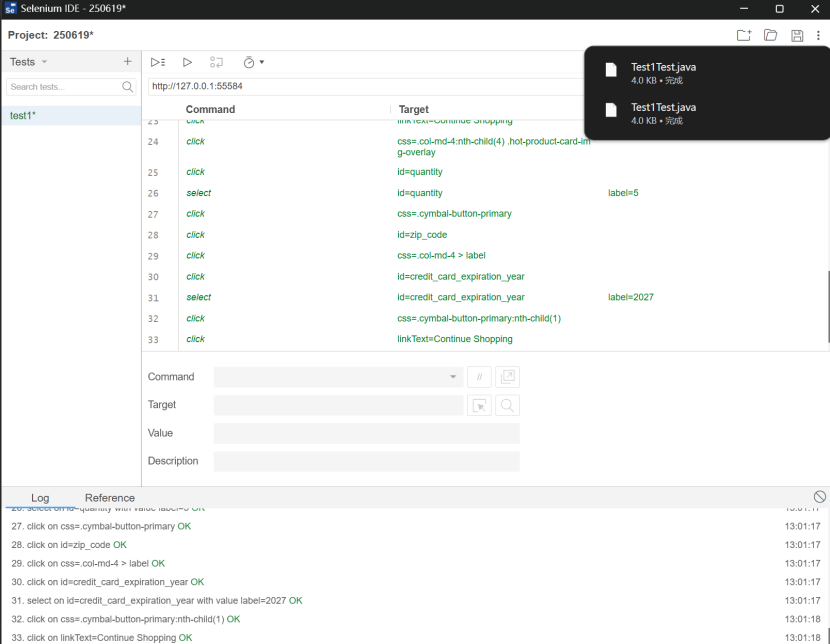
\includegraphics[width=0.75\linewidth]{测试/2.png}
    \label{fig:enter-label}
\end{figure}
将java脚本进行修改,以在Jmeter上运行,以下最后一次为修改后运行成功的记录
\begin{figure}[H]
    \centering
    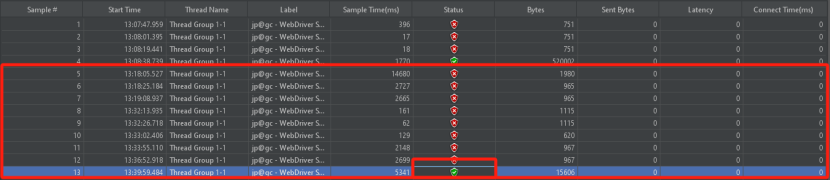
\includegraphics[width=0.75\linewidth]{测试/3.png}
    \label{fig:enter-label}
\end{figure}
调试修改合适的线程数、启动时间、循环时间
\begin{figure}[H]
    \centering
    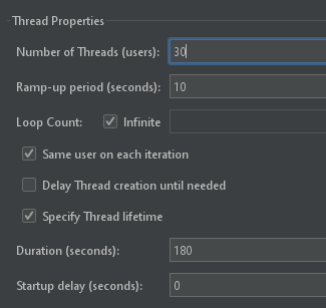
\includegraphics[width=0.75\linewidth]{测试/4.png}
    \label{fig:enter-label}
\end{figure}

运行,发现当线程数太多(>=50)时网站会出现connect: connection refused的错误,于是选择线程数为30,运行测试成功
\begin{figure}[H]
    \centering
    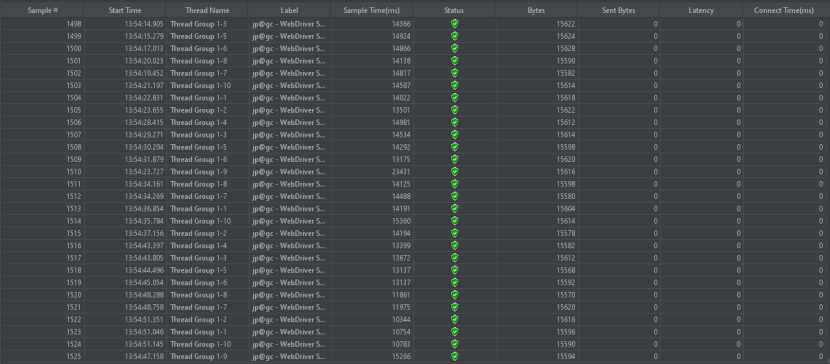
\includegraphics[width=0.75\linewidth]{测试/5.png}
    \label{fig:enter-label}
\end{figure}

Grafana捕获的数据在附录文件中

最后运行脚本,生成excel记录及html报告
\begin{figure}[H]
    \centering
    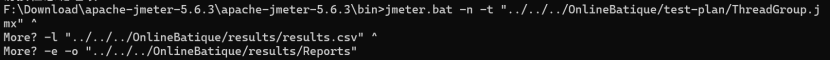
\includegraphics[width=0.75\linewidth]{测试/6.png}
    \label{fig:enter-label}
\end{figure}
\begin{figure}[H]
    \centering
    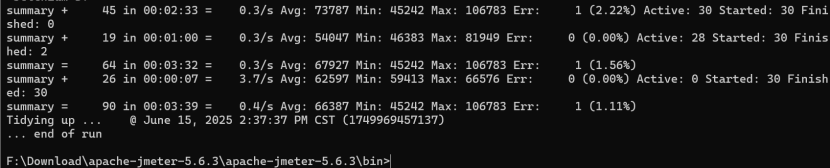
\includegraphics[width=0.75\linewidth]{测试/7e.png}
    \label{fig:enter-label}
\end{figure}
\begin{figure}[H]
    \centering
    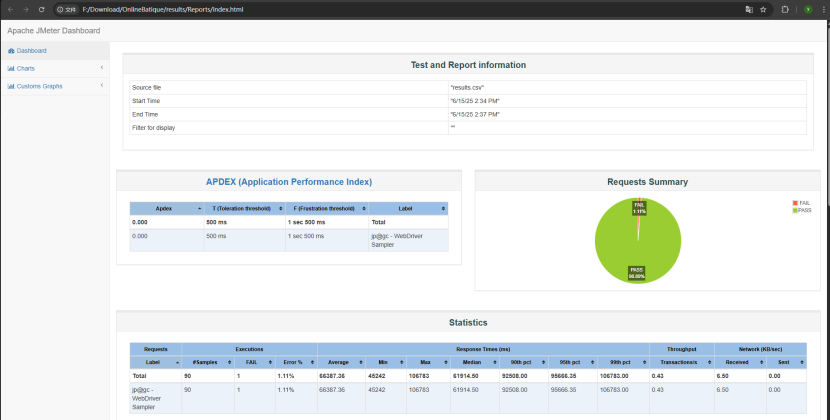
\includegraphics[width=0.75\linewidth]{html.png}
    \caption{HTML报告}
    \label{fig:enter-label}
\end{figure}
HTML报告具体内容在附录文件中

测试源代码如下:
\begin{lstlisting}
   import org.openqa.selenium.*
import org.openqa.selenium.support.ui.Select
import org.openqa.selenium.Dimension

// 已删除手动调用的 sampleStart()/sampleEnd()

WDS.browser.get("http://127.0.0.1:55584/")
WDS.browser.manage().window().setSize(new Dimension(922, 960))

// 选择商品
WDS.browser.findElement(By.cssSelector(".col-md-4:nth-child(2) .hot-product-card-img-overlay")).click()
WDS.browser.findElement(By.cssSelector("img:nth-child(2)")).click()

// 设置商品数量(修复:使用 Select 类)
Select quantitySelect = new Select(WDS.browser.findElement(By.id("quantity")))
quantitySelect.selectByVisibleText("10")  // 直接选择选项
WDS.browser.findElement(By.cssSelector(".cymbal-button-primary")).click()

// 结账流程
WDS.browser.findElement(By.cssSelector(".cymbal-button-primary:nth-child(1)")).click()
WDS.browser.findElement(By.linkText("Continue Shopping")).click()

// 第二件商品
WDS.browser.findElement(By.cssSelector(".col-md-4:nth-child(3) .hot-product-card-img-overlay")).click()
// 再次使用 Select 类
quantitySelect = new Select(WDS.browser.findElement(By.id("quantity")))
quantitySelect.selectByVisibleText("2")
WDS.browser.findElement(By.cssSelector(".cymbal-button-primary")).click()

// 支付信息(修复:使用 Select 类)
Select monthSelect = new Select(WDS.browser.findElement(By.id("credit_card_expiration_month")))
monthSelect.selectByVisibleText("August")
WDS.browser.findElement(By.cssSelector(".cymbal-button-primary:nth-child(1)")).click()
WDS.browser.findElement(By.linkText("Continue Shopping")).click()

// 货币切换(修复:使用 Select 类)
Select currencySelect = new Select(WDS.browser.findElement(By.name("currency_code")))
currencySelect.selectByVisibleText("JPY")
WDS.browser.findElement(By.cssSelector(".cart-link")).click()
WDS.browser.findElement(By.linkText("Continue Shopping")).click()

// 第三件商品
WDS.browser.findElement(By.cssSelector(".col-md-4:nth-child(4) .hot-product-card-img-overlay")).click()
quantitySelect = new Select(WDS.browser.findElement(By.id("quantity")))
quantitySelect.selectByVisibleText("5")
WDS.browser.findElement(By.cssSelector(".cymbal-button-primary")).click()

// 完成支付(修复:使用 Select 类)
WDS.browser.findElement(By.id("zip_code")).sendKeys("12345")  // 添加邮编输入
Select yearSelect = new Select(WDS.browser.findElement(By.id("credit_card_expiration_year")))
yearSelect.selectByVisibleText("2027")
WDS.browser.findElement(By.cssSelector(".cymbal-button-primary:nth-child(1)")).click()
  
\end{lstlisting}


\section{故障注入与监控}
为了测试微服务系统在面临突发故障时的鲁棒性与恢复能力,本实验引入了混沌工程工具 Chaos Mesh 对 Online Boutique 微服务平台进行故障注入与系统行为监控。Chaos Mesh 是一款专为 Kubernetes 环境设计的开源混沌工程平台,支持多种类型的故障模拟,包括 CPU 过载、内存耗尽、IO 延迟、网络丢包、Pod 终止等。通过模拟系统中的“非预期”行为,开发者可以观察系统在极端情况下的表现,从而提升架构的容错能力和稳定性。
实验中,首先通过 Helm 工具在 Kubernetes 集群中安装 Chaos Mesh,并通过获取 Dashboard 登录所需的 token,实现了在本地通过端口转发访问 Chaos Mesh 的可视化控制台。我们在实验中选取了三类典型的混沌实验类型,分别是 CPU 负载、IO 延迟以及 Pod Kill 故障。它们涵盖了计算资源、存储资源和服务可用性三个关键维度

\subsection{CPU负载故障}
该类故障通过模拟前端服务出现大量 CPU 和内存资源占用的场景,以此测试服务在高并发压力下的响应能力和稳定性。具体配置中,Chaos Mesh 启动了 20 个 CPU 工作线程,持续造成 80\% 的负载,同时还分配了 16 个线程对每个线程使用 2GB 内存,持续 120 秒。这种应激模拟常用于发现性能瓶颈、检测负载均衡配置效果以及前端 UI 层的容错策略是否生效,例如是否会触发错误提示或自动退回机制
\begin{lstlisting}
    kind: StressChaos
apiVersion: chaos-mesh.org/v1alpha1
metadata:
  namespace: default
  name: cpu-frontend-3
spec:
  selector:
    namespaces:
      - default
    labelSelectors:
      app: frontend
  mode: one
  stressors:
    memory:
      workers: 16
      size: 2G
    cpu:
      workers: 20
      load: 80
  duration: 120s
\end{lstlisting}
\subsubsection{反应结果}
反应结果如下图所示
\begin{figure}[H]
    \centering
    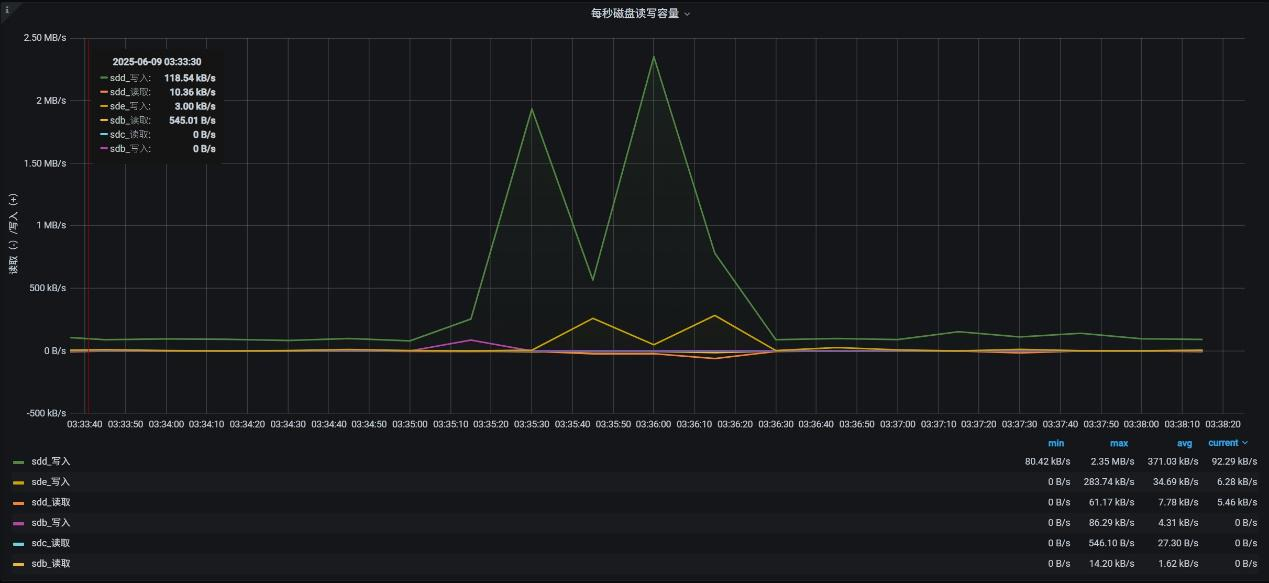
\includegraphics[width=0.75\linewidth]{故障注入/1.png}
    \caption{每秒磁盘读写容量}
    \label{fig:enter-label}
\end{figure}
\begin{figure}[H]
    \centering
    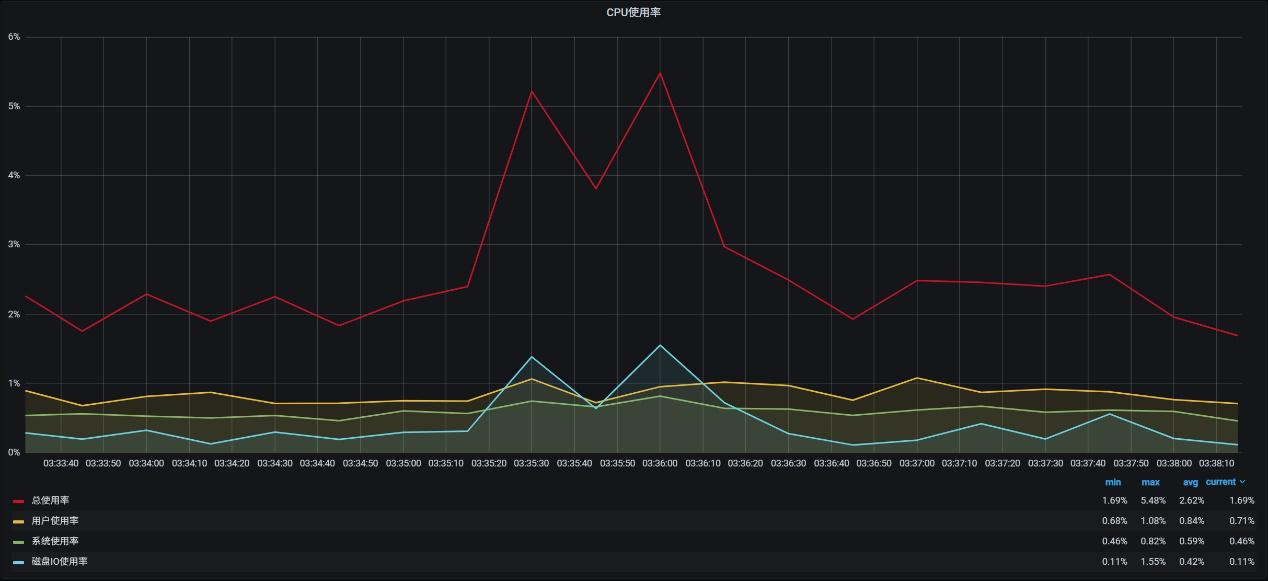
\includegraphics[width=0.75\linewidth]{故障注入/2.png}
    \caption{CPU使用率}
    \label{fig:enter-label}
\end{figure}
\begin{figure}[H]
    \centering
    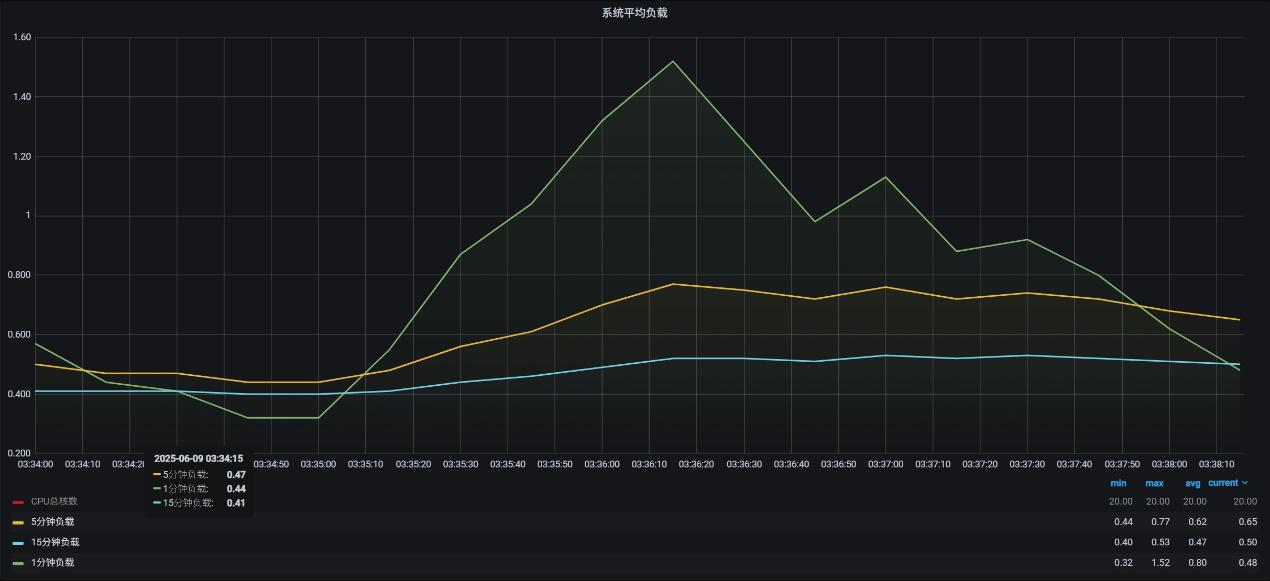
\includegraphics[width=0.75\linewidth]{故障注入/3.png}
    \caption{系统平均负载}
    \label{fig:enter-label}
\end{figure}
\subsubsection{结果分析}
\begin{enumerate}
    \item 使用率回落快速,说明系统资源充足,未出现资源争用或瓶颈。
    \item 负载增长稳定,无抖动,系统调度正常,负载处于健康可控区间,未造成严重阻塞。
    \item 系统可能发生了 swap 交换、临时缓存写入或日志记录增强。
\end{enumerate}

\subsection{IO注入故障}
在微服务架构中,磁盘读写速度对整体响应性能起到关键作用。我们选择对 productcatalogservice 服务引入磁盘延迟故障,模拟磁盘访问受阻的极端场景。配置中添加了 150ms 的 IO 延迟,生效范围为 100\%,即所有访问该服务的请求都会受到影响。这类故障有助于测试服务在磁盘慢速访问时是否存在缓存机制、是否会造成请求阻塞或超时,亦可进一步配合观察用户浏览商品详情时的体验变化。

\begin{lstlisting}
    kind: IOChaos
apiVersion: chaos-mesh.org/v1alpha1
metadata:
  namespace: default
  name: io-delay-pcatalog-1
  annotations:
    experiment.chaos-mesh.org/pause: 'true'
spec:
  selector:
    namespaces:
      - default
  mode: all
  action: latency
  delay: 150ms
  percent: 100
  volumePath: /data
  duration: 120s
\end{lstlisting}
\subsubsection{反应结果}
\begin{figure}[H]
    \centering
    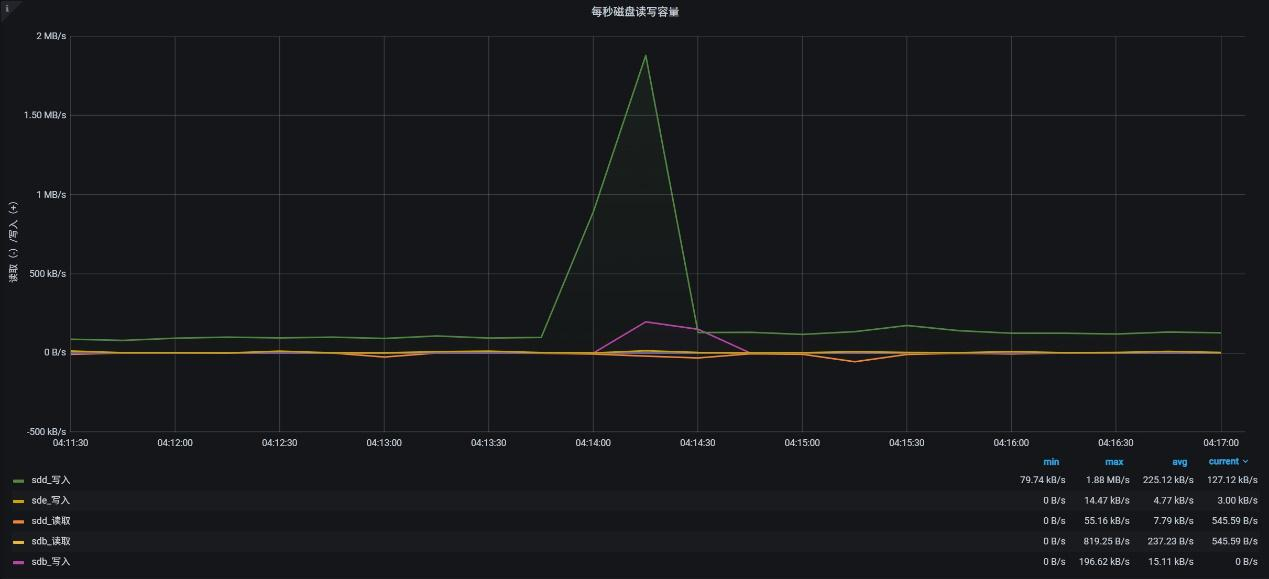
\includegraphics[width=0.75\linewidth]{故障注入/4.png}
    \caption{每秒磁盘读写容量}
    \label{fig:enter-label}
\end{figure}
\begin{figure}[H]
    \centering
    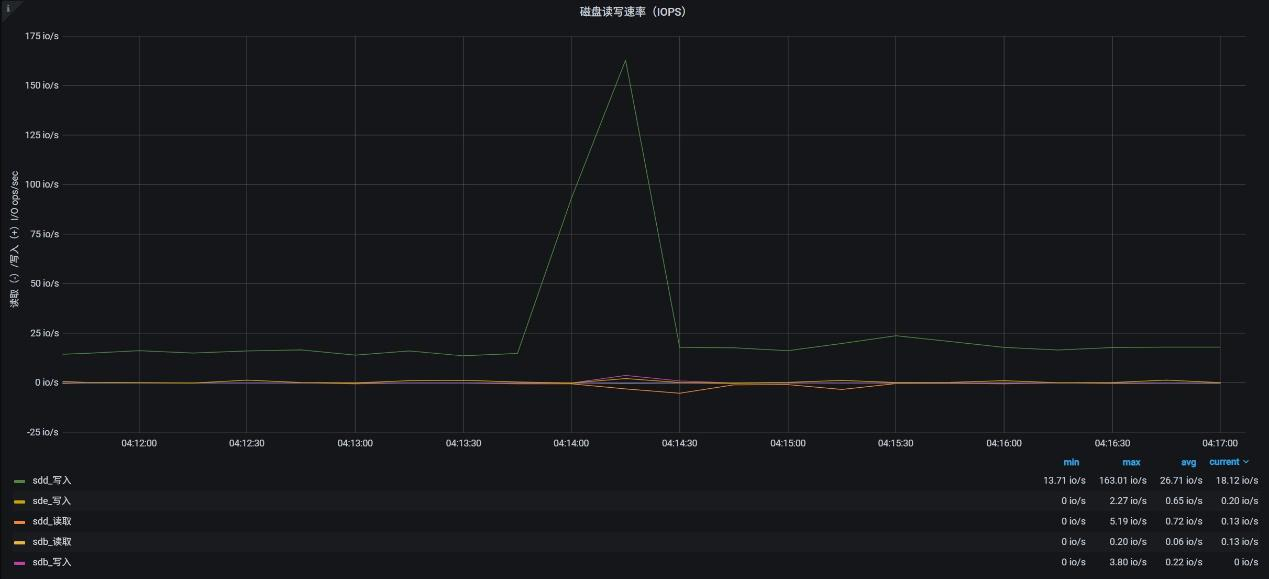
\includegraphics[width=0.75\linewidth]{故障注入/5.png}
    \caption{磁盘读写速率}
    \label{fig:enter-label}
\end{figure}
\begin{figure}[H]
    \centering
    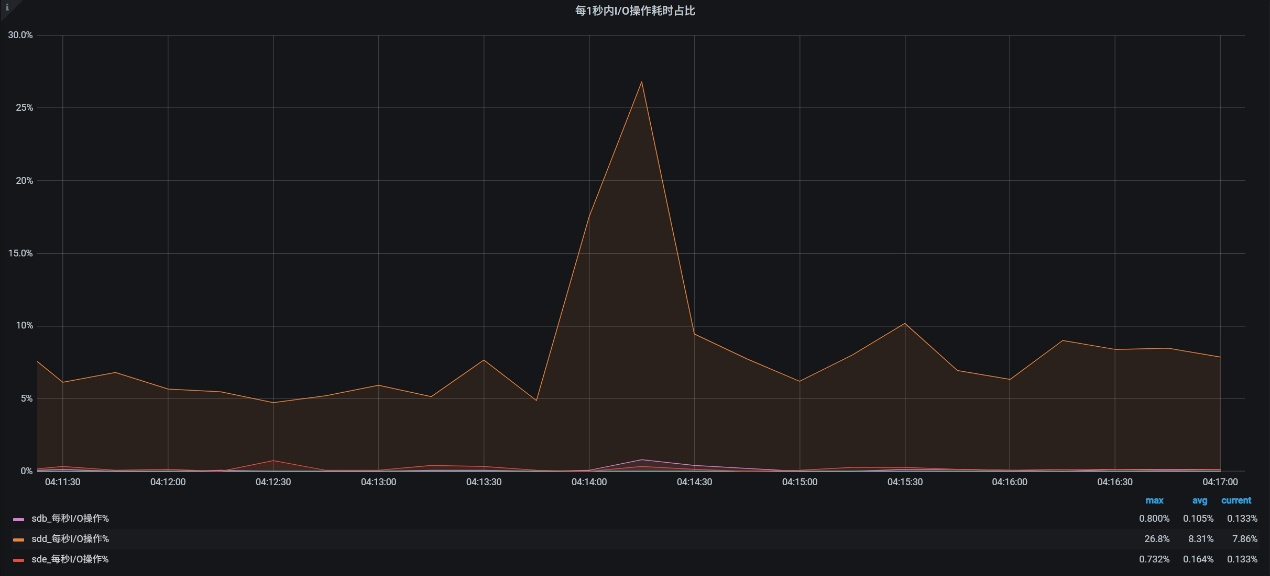
\includegraphics[width=0.75\linewidth]{故障注入/6.png}
    \caption{每1秒内I/O操作耗时占比}
    \label{fig:enter-label}
\end{figure}
\begin{figure}[H]
    \centering
    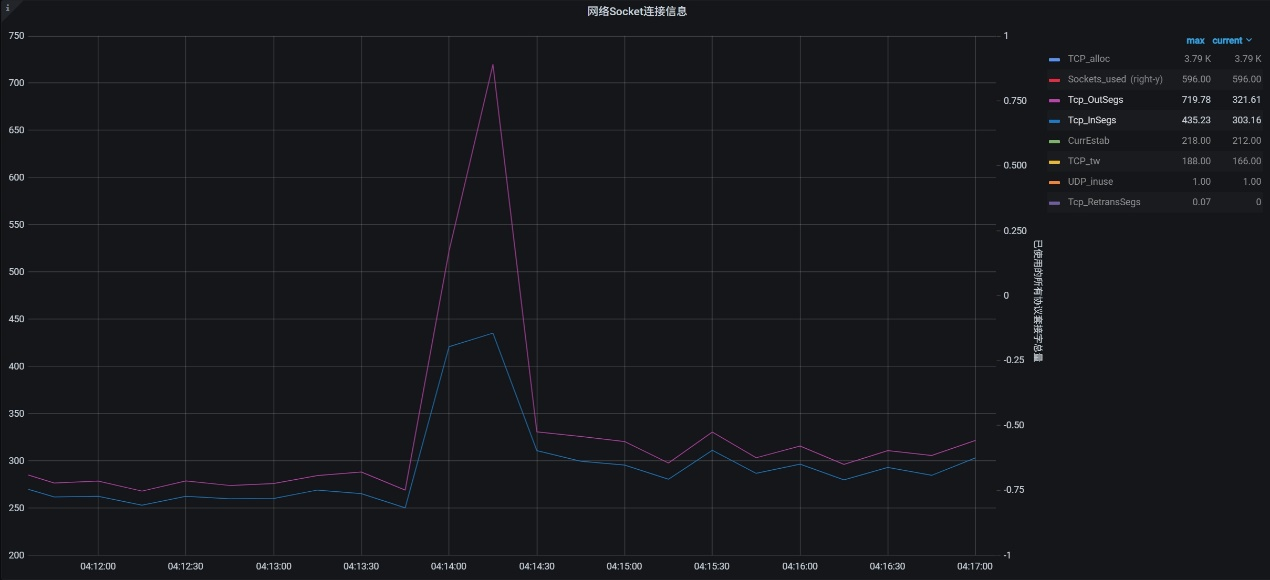
\includegraphics[width=0.75\linewidth]{故障注入/7.png}
    \caption{网络Socket连接信息}
    \label{fig:enter-label}
\end{figure}

\subsubsection{结果分析}
\begin{enumerate}
    \item 故障期间存在 IO 写入积压后集中释放的现象,磁盘响应能力受到干扰。
    \item 注入有效提升了磁盘操作次数,造成暂时性 IO 拥塞。
    \item 注入延迟确实导致系统在等待磁盘响应上的时间明显增加。
    \item 延迟影响了服务响应能力,导致 TCP 层短时流量变化,但连接层保持稳定,系统容错较强。
\end{enumerate}

\subsection{POD KILL}
Pod Kill 是最直接的模拟服务宕机方式。Chaos Mesh 会主动将某个服务 Pod 杀死,以验证 Kubernetes 的自动重启机制和副本调度能力是否健壮。在本实验中,我们对 productcatalogservice 服务执行了 Pod Kill 操作。在服务突发崩溃的情况下,系统应能快速重建 Pod 并恢复连接,若未设置副本数则会观察到前端服务商品无法加载的现象。这类实验适用于测试单点失效影响范围、负载均衡路由策略和服务健康检查机制。

\begin{lstlisting}
kind: PodChaos
apiVersion: chaos-mesh.org/v1alpha1
metadata:
  namespace: default
  name: podkill-product-1
spec:
  selector:
    namespaces:
      - default
    labelSelectors:
      app: productcatalogservice
  mode: one
  action: pod-kill
\end{lstlisting}
\subsubsection{反应结果}
\begin{figure}[H]
    \centering
    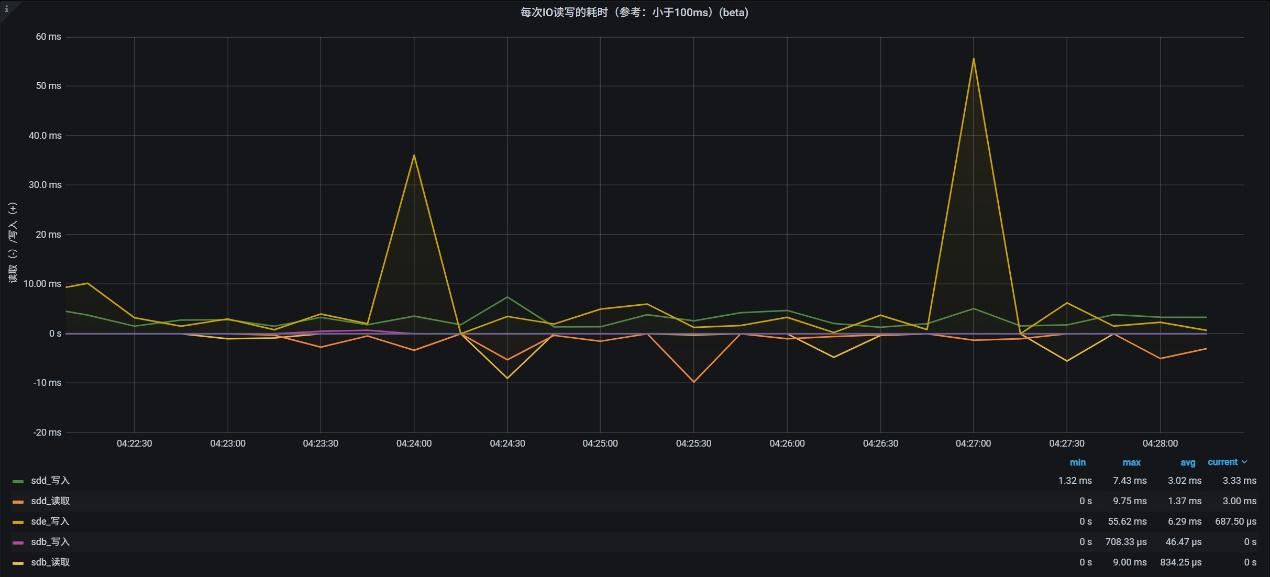
\includegraphics[width=0.75\linewidth]{故障注入/8.png}
    \caption{每次IO读写的耗时}
    \label{fig:enter-label}
\end{figure}

\subsubsection{结果分析}
\begin{itemize}
    \item 两次 Pod 被 Kill 后,磁盘写入出现瞬时延迟激增,说明服务重启过程触发了磁盘写操作。系统都在 1 分钟内完成了恢复。
\end{itemize}

\section{实验数据收集}
数据源自部署在 Kubernetes 微服务集群中的 11 个 POD,主要采集以下指标:
\subsection{Pod 级别指标}
\begin{enumerate}
    \item CPU 使用率
    \item 内核使用率
    \item 用户空间使用率
    \item 内存占用
    \item 最大内存使用量
    \item Pod 重启次数
\end{enumerate}

\subsection{系统级指标}
\begin{enumerate}
    \item 网络流量(接收/发送字节数与错误数)
    \item 磁盘空间使用与限制
    \item 磁盘 I/O 次数与耗时
\end{enumerate}

\subsection{数据处理方法}
\begin{enumerate}
    \item 训练集:仅使用正常运行数据,用于学习系统的“健康”行为模式
    \item 测试集:通过 Chaos Mesh 注入攻击进行标注(0 表示正常,1 表示异常)
    \item 特征标准化:所有特征进行归一化处理
    \item 划分比例:训练集与测试集时间段不重叠,确保评估的真实性与泛化能力
\end{enumerate}

\subsection{收集结果}
具体收集流程可参考源代码中的collect.py
收集到的数据如下:
\begin{figure}[H]
    \centering
    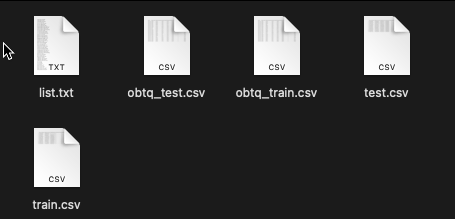
\includegraphics[width=0.75\linewidth]{数据收集/1.png}
    \label{fig:enter-label}
\end{figure}

\section{GDN论文复现}
本实验基于图偏差网络(Graph Deviation Network, GDN)对微服务系统的监控数据进行异常检测,复现了原论文的算法,并结合实际数据进行了对比分析。

\subsection{GDN图偏差网络算法关键点}
论文针对高维时间序列(如传感器数据)中的异常检测问题,提出了一种基于图神经网络的Graph Deviation Network (GDN) 方法。核心挑战在于如何显式建模传感器间的复杂非线性关系,并解释异常事件的偏离模式。
\subsubsection{传感器嵌入(Sensor Embedding)}
    为每个传感器引入独立的嵌入向量 viv\_ivi,以学习其潜在特性。相似嵌入代表传感器在功能或行为上的相关性,为后续图结构构建与注意力聚合提供基础。
\subsubsection{图结构学习(Graph Structure Learning)}
    通过学习动态图结构建模传感器间的关系。系统采用 Top-K 邻接策略为每个节点选择关键邻居,同时支持融合先验知识(如传感器物理位置或服务关系),提升图结构语义。
\subsubsection{图注意力预测(Graph Attention Prediction)}
    在已构建图结构的基础上,使用图注意力机制对邻居节点信息加权聚合,实现对每个传感器未来状态的预测。该机制提升了模型对局部异常的感知能力。
\subsubsection{图偏差评分(Graph Deviation Scoring)}
    计算每个传感器预测值与实际值之间的偏差,并通过中位数与四分位距(IQR)归一化,以最大偏差作为整体异常分数。最终通过平滑与设定阈值进行异常判定。
\begin{figure}[H]
    \centering
    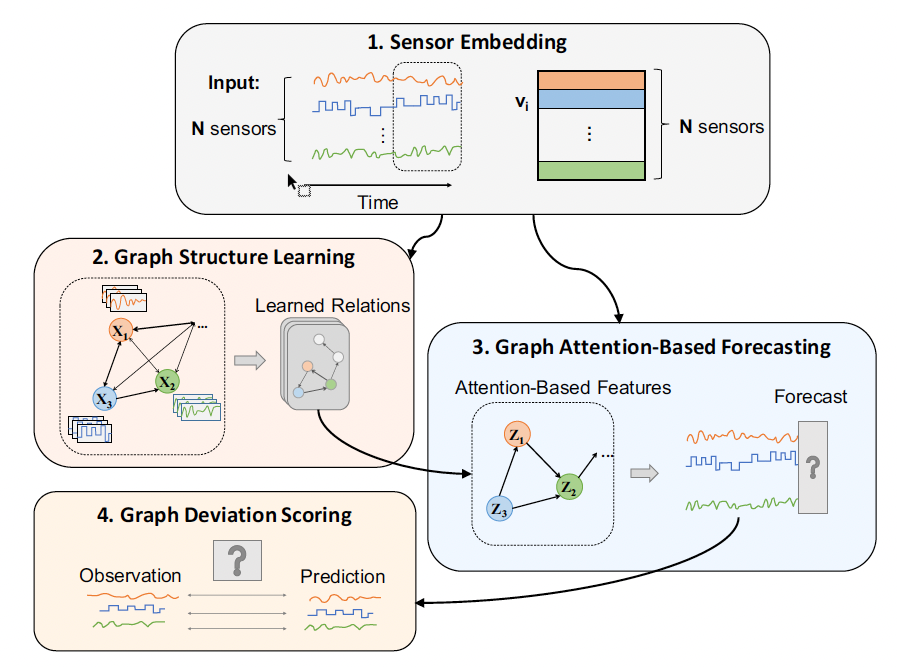
\includegraphics[width=0.75\linewidth]{图偏差网络框架图.png}
    \caption{GDN框架图}
    \label{fig:enter-label}
\end{figure}

\subsection{复现过程及结果}
环境准备
运行安装脚本 install\_cpu.sh 或 install.sh 完成依赖安装。
\begin{figure}
    \centering
    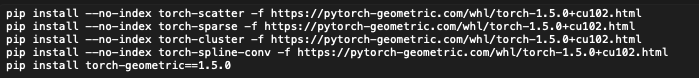
\includegraphics[width=0.75\linewidth]{复现/install.png}
    \label{fig:enter-label}
\end{figure}
数据准备
数据集结构遵循 data/<dataset\_name>/ 格式,包含 list.txt、train.csv 和 test.csv
确保 test.csv 包含 attack 列作为标签
\begin{figure}
    \centering
    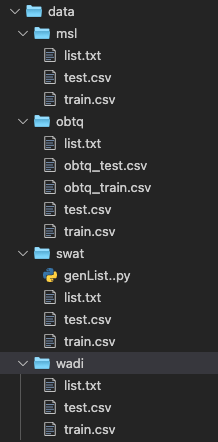
\includegraphics[width=0.25\linewidth]{复现/dataset.png}
    \caption{数据准备}
    \label{fig:enter-label}
\end{figure}

运行模型
使用 run.sh 脚本启动训练与测试,支持 CPU 和 GPU 模式。
\begin{figure}[H]
    \centering
    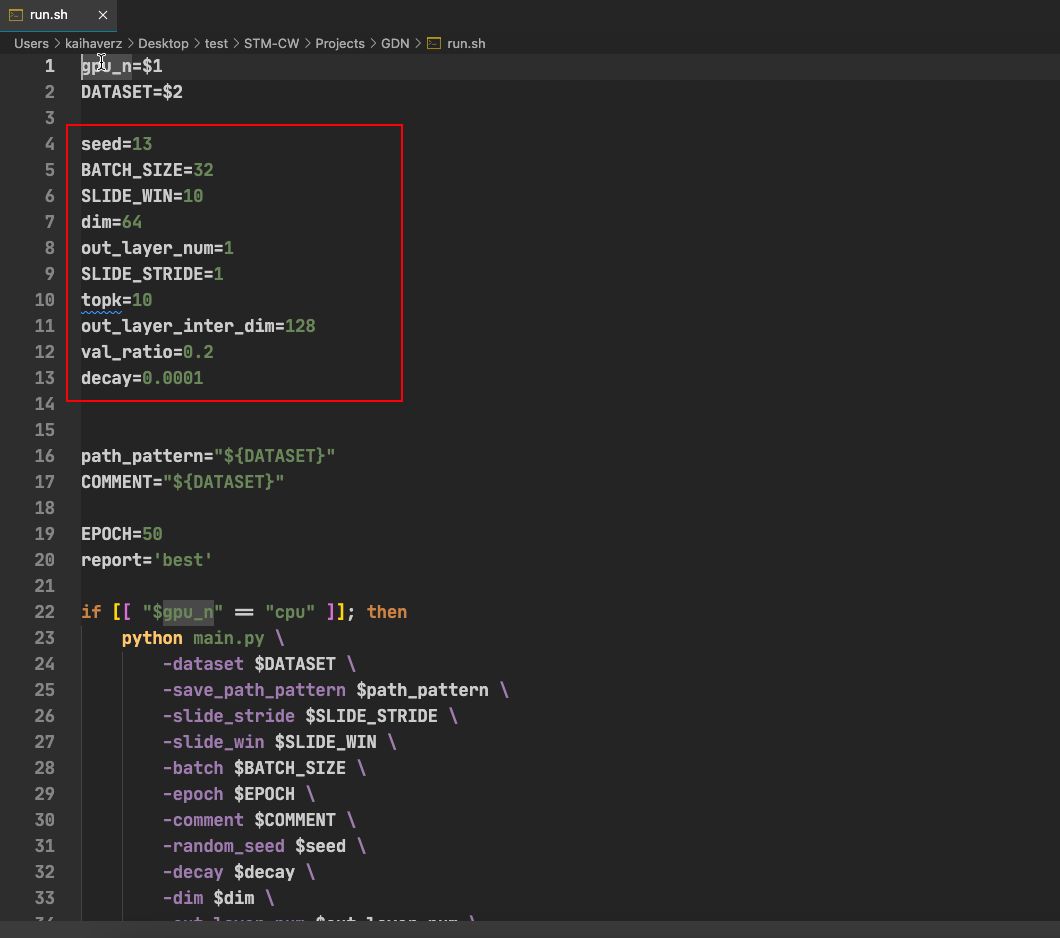
\includegraphics[width=0.75\linewidth]{复现/run.png}
    \caption{run.sh}
    \label{fig:enter-label}
\end{figure}
关键参数配置如下:
\begin{itemize}
    \item BATCH\_SIZE=32
    \item SLIDE\_WIN=10
    \item dim=64
    \item EPOCH=50
\end{itemize}
\begin{figure}[H]
    \centering
    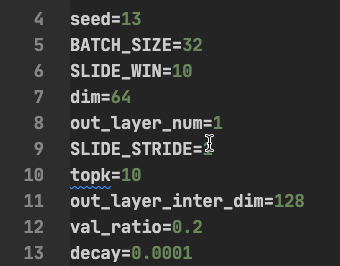
\includegraphics[width=0.75\linewidth]{复现/关键参数.png}
    \caption{关键参数设置}
    \label{fig:enter-label}
\end{figure}

复现结果:
\begin{figure}[H]
    \centering
    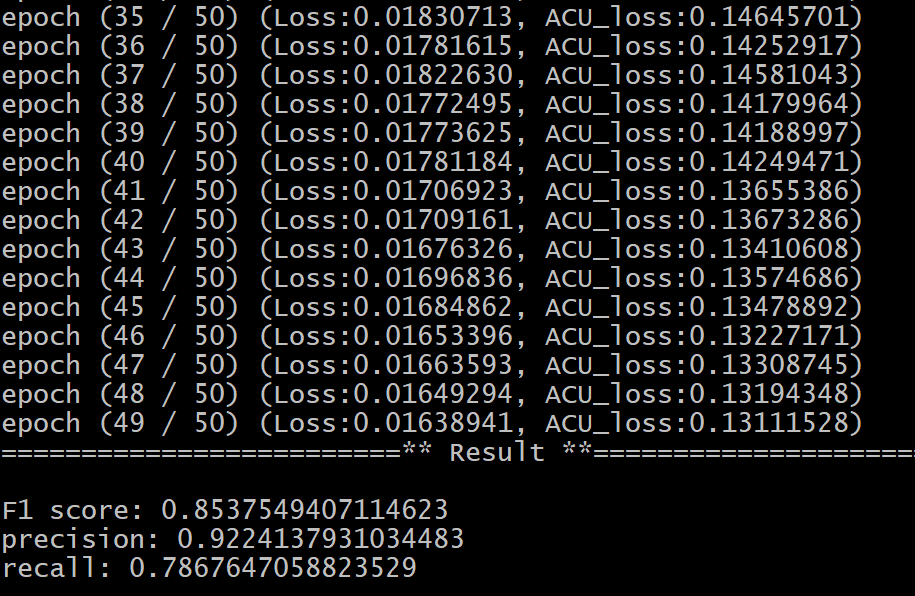
\includegraphics[width=0.75\linewidth]{复现/result.png}
    \caption{复现结果}
    \label{fig:enter-label}
\end{figure}
\begin{itemize}
    \item F1 score: 0.8537549407114623
    \item precision: 0.9224137931034483
    \item recall: 0.7867647058823529
\end{itemize}


\subsection{复现结果分析}
\begin{figure}
    \centering
    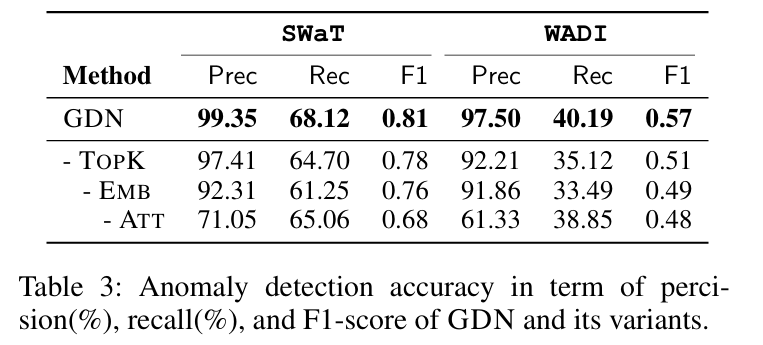
\includegraphics[width=0.75\linewidth]{复现/论文结果.png}
    \caption{原论文结果}
    \label{fig:enter-label}
\end{figure}
本次实验复现结果,准确率指标与原论文存在一定差距,经分析,可能的原因如下:
\subsubsection{数据规模差异显著}
原论文构建训练集时,采集了水处理厂连续两周的监控数据,总样本量达十万余条。而本组复现实验受客观条件限制,仅采集了微服务系统几小时内的千条数据,可能导致模型对数据分布的学习不充分,从而影响预测精度与泛化能力
\subsubsection{数据特性存在本质差异}
原论文数据来源于水处理厂,数据特征相对稳定,变量间的关联模式遵循固定的物理或化学规律(如水温、水压与流量的联动关系)。而本次实验数据采集自微服务系统,该系统具有高动态性与复杂交互性,数据分布的复杂性显著增加,使得原论文模型在新场景下的适配性降低。
\subsubsection{数据标注存在局限性}
标注误差不可避免:测试集的异常标签采用人工标注方式,因注入故障时间的差异,难免引入标注误差
标注覆盖不全:本次标注仅针对注入式故障(如人为模拟的资源耗尽),未能覆盖非注入式异常(如服务间依赖冲突、代码逻辑错误引发的性能下降)。这种标注偏差使模型难以识别实际运行中的复杂异常模式,造成漏检或误报现象。


\section{实验总结及展望}
\subsection{总结}
本实验以 Google 开源微服务项目 Online Boutique 为基础,系统性地开展了从微服务架构部署到性能测试、混沌工程、监控可观测性建设及智能异常检测算法复现的全流程实践。通过 Minikube 在本地部署 Kubernetes 环境,成功实现了多语言微服务的容器化管理与集群调度,直观体验了微服务架构的解耦、弹性与可维护性优势。在此基础上,利用 JMeter 和 Selenium 对系统进行了压力与自动化测试,验证了系统在并发场景下的稳定性与响应能力。
同时,实验引入 Chaos Mesh 实现了三类典型故障注入(CPU 过载、IO 延迟、Pod Kill),真实模拟运维中可能遇到的问题,强化了对系统鲁棒性、自动恢复机制及微服务之间容错协作能力的理解。此外,借助 Prometheus 和 Grafana 构建可视化监控系统,全面掌握了云原生环境中的指标采集与分析流程。
最后,结合 GDN(Graph Deviation Network)论文复现任务,将理论研究与系统实践结合,通过图神经网络模型对监控数据进行异常检测,有效提升了实验的智能化水平。该部分训练与测试过程不仅加深了对 AI 算法在分布式系统运维中的应用理解,也增强了对监控数据建模、图结构学习与异常评分机制的掌握。

\subsection{展望}
本实验在掌握微服务系统构建与运维的基础上,为未来的研究与开发积累了丰富的经验与工具链。展望后续工作,可从以下几个方向进一步深化:
智能监控能力提升:将更多先进的时间序列预测模型(如 Transformer、LSTM-FCN)引入异常检测模块,提升对复杂场景下系统行为的识别能力。
多故障协同模拟:在现有故障注入基础上,探索更复杂的多种故障联动场景,评估系统在多维应激下的恢复机制和性能边界。
跨集群部署与混合云支持:将部署环境拓展到远程 Kubernetes 集群(如 GKE、阿里云 ACK 等),研究在实际云平台下资源调度、网络通信与成本优化策略。
CI/CD 与 DevOps 融合:集成 GitHub Actions、ArgoCD 等工具实现自动化部署与版本控制,推动从实验系统向工业级持续集成体系转化。
微服务安全性研究:引入服务网格(如 Istio)实现服务间的身份认证与访问控制,进一步探索微服务环境下的安全治理机制。

\end{document}
